\introsection{Магнитное поле в веществе}

Известно, что вещество может обладать как собственной намагниченностью, так
и изменять свою намагниченность при помещении во внешнее магнитное поле.
Микроскопическими источниками магнитного поля в среде являются
орбитальное движение электронов в молекулах и атомах, а также собственное 
вращение (спин) электронов и ядер.
При \emph{макроскопическом} описании свойств среды, можно считать,
что каждый элемент объёма среды может являться элементарным источником
магнитного поля --- \emph{магнитным диполем}. Для описания усреднённых
свойств среды используют \term{вектор намагниченности} $\vec{M}$, равный
\important{магнитному моменту единичного объёма вещества} 
(объёмная плотность магнитного момента, размерность в 
системе СИ $[M]=\frac{А\cdot м^2}{м^3}=\frac{А}{м}$).

Магнитное поле на микроскопическом уровне (на масштабах атомов) 
$\vec{B}_{\text{микро}}$ испытывает резкие изменения в пространстве.
Величина магнитного поля $\vec{B}$ в данной точке среды определяется как
значение микрополя, усреднённое по малому (элементарному) объёму, 
содержащему при этом большое количество частиц: 
$\vec{B}=\lim\limits_{\Delta V\to 0}\int_{\Delta V} \vec{B}_{микро}dV$.
По историческим причинам вектор $\vec{B}$ 
называют \term{индукцией поля} (размерность $[B] = \frac{Н}{А\cdot м}\equiv  Тл$).

Помимо этого, принято вводить вспомогательный вектор $\vec{H}$
(\term{напря\-жённость поля}, $[H]=\frac{А}{м}$), определяемый 
из соотношения
\begin{equation}
    \eqmark{fieldB}
    \vec{B} = \mu_0(\vec{H} + \vec{M}),
\end{equation}
где $\mu_0=4\pi \cdot 10^{-7}\;\frac{Н}{А^2}$ --- магнитная постоянная.

В простейшем практически важном случае намагниченность $\vec{M}$ в каждой
точке среды прямо пропорциональна вектору напряжённости магнитного
поля~$\vec{H}$ в этой же точке:
\begin{equation}
    \eqmark{magnetization}
    \vec{M} = \chi\vec{H}.
\end{equation}
Коэффициент $\chi$ называют \term{магнитной восприимчивостью} среды.
Вещества, для которых закон \eqref{magnetization} выполняется
с хорошей точностью, называют \term{парамагнетиками} ($\chi > 0$) и
\term{диамагнетиками} ($\chi < 0$).
В~парамагнетиках элементарные диполи
ориентированы в основном по приложенному полю,
а в диамагнетиках --- против него.

Если закон \eqref{magnetization} применим,
то можно записать
\begin{equation}
    \vec{B} = \mu\mu_0 \vec{H},\qquad \text{где }\mu = 1 + \chi\text{~---}
\end{equation}
--- \term{магнитная проницаемость} вещества%
\footnote{В системе СГС имеют место соотношения
    $\vec{B}=\vec{H}+4\pi\vec{M}=\mu\vec{H}$, $\mu = 1 + 4\pi \chi$.}.

Отметим, что соотношение \eqref{magnetization} отнюдь не универсально. 
В~общем случае зависимость $\vec{M}(\vec{H})$ может быть \emph{нелинейной}, 
а также зависеть от <<предыстории>> образца ---
значений полей в предыдущие моменты времени
(явление \emph{гистерезиса} в ферромагнетиках).

\introsection{Свойства магнитных сред}

Полноценное рассмотрение магнитных свойств электронов и ядер
возможно только с использованием квантовой механики. 
В этом разделе мы ограничимся рассмотрением
упрощённых полуклассических моделей --- они
наглядны и дают правильные по порядку величины результаты.

\introsubsection{Диамагнетизм}
\label{sec:diamagnetism}

Диамагнетизм ($\chi <0$) возникает из-за электромагнитной индукции 
молекулярных токов в электронных оболочках атомов,
и присущ в той или иной степени всем веществам без исключения.

\paragraph{Случай $L=0$}
Рассмотрим электрон в атоме, находящийся в состоянии с нулевым
орбитальным моментом импульса $L=0$ ($s$-состояние). Соответствующий магнитный
момент также равен нулю $\mathsf{m}_L = 0$ (собственный, т.\,е. спиновый,
момент электрона рассматривать не будем).
С~классической точки зрения такое состояние можно представить как симметрично
<<размазанное>> облако заряда вокруг ядра.
% Пусть средний радиус облака равен $a$, масса электрона $m_e$, заряд $-e$.

Плавно (квазистатически) включим внешнее однородное магнитное поле~$\vec{B}$.
Под действием вихревого электрического поля~$\vec{E}$, 
возникающего из-за наличия переменного магнитного поля, 
электронное облако придёт во вращение.
Согласно закону электромагнитной индукции, величина этого поля на расстоянии~$r$ 
от оси системы определяется соотношением
\begin{equation*}
2\pi r E = - \pi r^2 \frac{dB}{dt}\qquad \to \qquad E = - \frac12 r\frac{dB}{dt}.
\end{equation*}
Запишем уравнение моментов для точечного электрона,
находящегося на <<орбите>> радиуса~$r$:
\begin{equation}
m_e r^2 \frac{d\omega}{dt} = - e r E = \frac12 er^2\frac{dB}{dt}.
\eqmark{domega_dt}
\end{equation}
Интегрируя по времени \eqref{domega_dt}, найдём, 
что независимо от расстояния~$r$ электрон при
включении поля~$B$ приобретает угловую скорость вращения
\begin{equation}
    \eqmark{Larmor-Omega}
    \omega_L = \frac{eB}{2m_e}.
\end{equation}
Величину $\omega_L$ называют \term{ларморовской} частотой
(заметим, что она вдвое меньше циклотронной $\omega_B=eB/m$,
см. Раздел~III).

При вращении с ларморовской частотой электрон создаёт магнитное поле,
равное полю витка с током $I_L = e \frac{\omega_L}{2\pi}$.
Этот ток в свою очередь создаёт магнитный момент
\begin{equation*}
  \mathsf{m}_L = I_L \cdot S = - \frac{e^2 S}{4\pi m_e}B,
\end{equation*}
где $S$~--- площадь эквивалентного витка.
Примем для оценки $S\sim \pi a^2$, где $a$~--- среднее расстояние 
электронов до ядра.
%(аккуратный учёт сферической симметрии электронного облака
%даёт поправочный множитель $2/3$: $S=\frac23 \pi \left<r^2\right>$).
Тогда, для атома, содержащего~$Z$ электронов, имеем намагниченность среды
$M=Zn\cdot \Delta \mathsf{m}_L$, где $n$~--- число атомов в единице объема.
Отсюда находим оценку для магнитной
восприимчивости диамагнетиков:
\begin{equation}
    \eqmark{chi-dia}
\chi_{диа} \sim - \mu_0 \frac{e^2 a^2}{4 m_e} Z n.
\end{equation}

Взяв характерные для твердых тел значения
$a \sim 2 \cdot 10^{-10}$~м, $n\sim a^{-3} \sim 10^{29}\;м^{-3}$, 
получим, что $\chi_{диа} \sim - 10^{-6}~Z$. Эта оценка довольно груба,
но даёт правильные по порядку величины результаты
(например, для $^{30}$Zn: $\chi \approx -1,25\cdot 10^{-5}$).

\paragraph{Случай $L\ne0$}

Рассмотрим теперь случай, когда электрон исходно обладает некоторым
орбитальным моментом импульса $L=mvr$. 
Пусть вектор момента импульса $\vec{L}$ лежит в плоскости
рис.~\figref{electron orbit} и направлен под углом $\theta$ к некоторой оси $z$.
Орбитальное движение электрона эквивалентно витку с током,
магнитный момент которого $\vec{\mathsf{m}}_L$ пропорционален $\vec{L}$
и направлен против него (т.\,к. $e<0$).
Его величину можно найти как произведения тока $e\cdot \frac{v}{2\pi r}$ 
на площадь <<витка>> $\pi r^2$: $\mathsf{m}_L= \frac12 evr$.
При включении внешнего магнитного поля~$B$,
направленного вдоль~$z$, на электрон начинает
действовать момент силы $\vec{\mathsf{m}}_L\times \vec{B}$,
%перпендикулярный плоскости рис.~\figref{electron orbit} и направленный от
%нас. 
и уравнение движения электрона (уравнение моментов) будет иметь вид
\begin{equation}
\eqmark{mu_precession}
	\frac{d\vec{L}}{dt} = \vec{\mathsf{m}}_L\times \vec{B}.
\end{equation}

\begin{figure}[h!]
    \centering
    \pic{21mm}{Chapter_4/v4_1}
    \caption{Прецессия электронной орбиты в магнитном поле}
    \figmark{electron orbit}
\end{figure}

Как известно из механики, уравнение \eqref{mu_precession} 
описывает движение симметричного волчка (гироскопа). Его решением является
\emph{прецессия} электронной орбиты с \emph{ларморовской} угловой частотой:
$\omega_L = \frac{\mathsf{m}_L B}{L} = \frac{eB}{2m_e}$.
При этом вектор $\vec{\mathsf{m}}_L$ описывает конус вокруг вектора~$\vec{B}$.
%Подставляя значения $L$ и $\mathsf{m}_L$, находим
%$\omega_L = \frac{eB}{2m_e}$.
Эта прецессия не зависит от угла $\theta$ и приводит к дополнительному 
вращению электрона вокруг поля~$\vec{B}$, налагающемуся на его орбитальное 
движение. Нетрудно убедиться, что она даёт полностью аналогичный 
\eqref{chi-dia} вклад в диамагнитную восприимчивость.

% Сложно и ненужно // ППВ
%
% Если рассматривать сферически-симметричное распределение заряда
% электрона, то расчёт показывает, что $S = 2/3\pi\average{r^2}$, где
% $\average{r^2}$~--- средний квадрат расстояния электрона от ядра. Поэтому
% \begin{equation*}
% 	\Delta\mu = - \frac{\mu_0 e^2 \average{r^2}}{6m_e}H.
% \end{equation*}
%
% Появление этого момента и приводит к намагничиванию вещества в направлении,
% противоположном полю, т.е. к диамагнетизму. Магнитный момент атома, содержащего
% $Z$ электронов, находится суммированием магнитных моментов отдельных электронов:
% \begin{equation*}
% 	\mu_{\text{ат}} = - \frac{\mu_0 e^2 H}{6m_e}\sum\limits_{i=1}^Z
% \average{r_i^2}.
% \end{equation*}
%
% Сумму можно заменить произведением $Z\average{a^2}$, где $\average{a^2}$~---
% средний квадрат расстояния электронов от ядра. Тогда
% \begin{equation*}
% 	\mu_{\text{ат}} = - \frac{\mu_0 e^2 \average{a^2} Z}{6m_e}H.
% \end{equation*}
% Умножив полученное выражение на число атомов $n$ в единице объёма, получим
% намагниченность $M$:
% \begin{equation*}
% 	M = n\mu_{\text{ат}} = - \frac{\mu_0 e^2 \average{a^2} nZ}{6m_e}H.
% \end{equation*}
% Магнитная восприимчивость
% \begin{equation*}
% 	\chi = \frac{M}{H} = - \frac{\mu_0 e^2 \average{a^2} nZ}{6m_e}.
% \end{equation*}


Из выражения \eqref{chi-dia} следует, что диамагнитная восприимчивость 
не зависит от температуры или величины поля,
и возрастает пропорционально порядковому номеру элемента.
Видно, что диамагнитный эффект присущ всем веществам не зависимо от того, 
имеется ли у атомов собственный магнитный момент, или нет. Однако у некоторых 
веществ он перекрывается более сильным \emph{парамагнитным} эффектом.


\introsubsection{Парамагнетизм}
\label{sec:paramagnetism}

Парамагнетизм ($\chi>0$) характерен для веществ, микроскопические частицы которых 
(атомы, ионы, молекулы) обладают \emph{собственным} магнитным 
моментом в отсутствие внешнего магнитного поля.

В парамагнетиках энергия взаимодействия между соседними магнитными моментами
атомов мала по сравнению с тепловой энергией,
поэтому в отсутствие внешнего магнитного поля микроскопические магнитные моменты
полностью разупорядочены, и намагниченность среды равна нулю.
При помещении во внешнее поле магнитным моментам энергетически выгодно
ориентироваться преимущественно по полю, что и приводит к парамагнитному эффекту.

% Ненужные подробности // ППВ
%
% Этот магнитный момент обусловлен как движением электронов в оболочке атома
% (орбитальный магнитный момент), так и наличием собственных магнитных моментов
% у электронов и ядер (\term{спиновый} магнитный момент).
% Например, в кристаллах медного купороса (CuSO$_4$) содержатся ионы меди,
% у которых электроны на внутренних оболочках имеют суммарный магнитный момент,
% не равный нулю. Изолированный атом меди имеет
% нечётное число электронов (29). На внешней оболочке $4s$ имеется всего один
% электрон, и именно его магнитный момент является магнитным моментом атома меди.
% Поэтому пары меди, как и пары натрия, являются парамагнетиками. Однако при
% переходе в твёрдое состояние (в процессе кристаллизации) атомы меди теряют этот
% электрон, он уходит от своего атома и уже принадлежит всему кристаллу.
% «Застывшие» в узлах решётки ионы меди уже не имеют магнитного момента и поэтому
% не обладают парамагнитным эффектом. Обобществлённые электроны (электроны
% проводимости) образуют электронный газ, который является парамагнетиком,
% поскольку состоит из частиц, обладающих собственным магнитным моментом. Такой
% парамагнетизм называют \term{парамагнетизмом Паули}. Но медь является
% диамагнетиком, и это означает, что диамагнетизм ионов меди преобладает над
% парамагнетизмом свободных электронов.

% Отличительной особенностью парамагнетиков является их слабая намагниченность во
% внешнем магнитном поле при комнатной температуре. В отсутствие магнитного поля
% энергия диполь-дипольного взаимодействия между двумя соседними магнитными
% моментами атомов с межатомным расстоянием $\sim 5 \cdot 10^{-8}$~см составляет
% $\sim 10^{-5}$~эВ, а энергия
% теплового движения на атом $\sim 7,5 \cdot 10^{-2}$~эВ. Такое превосходство
% тепловой энергии приводит к равномерному пространственному распределению
% магнитных моментов, а следовательно, к отсутствию намагниченности у
% парамагнетиков. Но когда начинает действовать внешнее магнитное поле, оно
% выстраивает магнитные моменты так, что магнитных моментов, направленных по полю,
% становится больше, чем направленных против поля, и с ростом поля намагниченность
% парамагнетиков растёт по закону \eqref{magnetization-magnetic vector}.
% Магнитная восприимчивость парамагнетиков всегда положительна, а по величине
% $\chi \sim 10^{-6} \sim 10^{-4}$~(система СИ).

% Упростим вывод до предела!

Оценим температурную зависимость магнитной восприимчивости парамагнетика
в классической модели.
Пусть среднее число атомов в единице объёма равно~$n$, а абсолютная величина
магнитного момента атома~$\mathsf{m}_{\text{а}}$.
В магнитном поле с индукцией~$B$ энергия магнитного диполя,
составляющего с направлением поля угол $\alpha$, равна
\begin{equation*}
	U = - \mathsf{m}_{\text{а}}B \cos \alpha
\end{equation*}
и может меняться в диапазоне от $-\mathsf{m}_{а}B$ до $+\mathsf{m}_{а}B$.
%(квантовая механика говорит, что энергия может принимать
%ряд дискретных значений в этом же диапазоне).

% \begin{wrapfigure}[]{r}{0.35\textwidth}
% \centering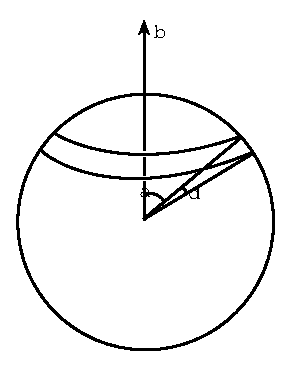
\includegraphics[width=0.2\textwidth]{v4_2}
% 	\caption{Телесный угол $d\Omega$.}
% 	\figmark{dN in dOmega}
% \end{wrapfigure}

Из термодинамики известно, что доля атомов $dn$, обладающих 
в условиях равносия энергией $U(\alpha)$, определяется распределением Больцмана:
\begin{equation*}
    dn \propto  e^{-\tfrac{U(\alpha)}{\kB T}} d\alpha.
\end{equation*}
Пусть внешнее магнитное поле достаточно мало,
так что энергия магнитных моментов атомов в
нём много меньше тепловой: $\mathsf{m}_{а}B \ll \kB T$.%
Число атомов, имеющих положительную ($\alpha > 0$) проекцию на направление~$\vec{B}$, может
быть записано как
\begin{equation*}
n_{+} = n_0 e^{\mathsf{m}_{а}B/\kB T}\approx n_0\left(1+\frac{\mathsf{m}_{а} B}{\kB T}\right),
\end{equation*}
где мы воспользовались разложением экспоненты от малого параметра,
а $n_0$ --- некоторая нормировочная константа. 
Для атомов с отрицательной проекцией момента ($\alpha < 0$):
\begin{equation*}
n_{-} = n_0 e^{-\mathsf{m}_{а}B/\kB T}\approx n_0\left(1-\frac{\mathsf{m}_{а} B}{\kB T}\right)
\end{equation*}
Учитывая условие нормировки $n_{+} + n_{-} = n$, найдём $n_0 \approx n/2$.

Суммарный магнитный момент единицы объёма можно оценить как
\begin{equation*}
M \sim n_{+}\mathsf{m}_{а} + n_{-}\cdot (-\mathsf{m}_{а}) \approx
\frac{\mathsf{m}_{а}^2 n}{\kB T} B.
\end{equation*}
Более аккуратное усреднение по углам даст поправочный множитель порядка единицы
(в классической модели получается коэффициент~$1/3$).

Таким образом, парамагнитная восприимчивость равна
\begin{equation}
    \eqmark{chi-para}
    \chi_{пар} \sim \mu_0 \frac{\mathsf{m}_{\text{а}}^2 n}{3\kB T}\propto \frac{1}{T}.
\end{equation}
Температурная зависимость восприимчивости парамагнетиков вида \eqref{chi-para}
называется \term{законом Кюри}. 

% Сложный вывод, при том нестрогий!
%
% Число атомов, магнитные моменты которых направлены под углами
% от $\alpha$ до
% $\alpha + d\alpha$ к полю, определяется распределением Больцмана:
% \begin{equation*}
%     dn = n_0 e^{-\tfrac{U}{\kB T}} \frac{d\Omega}{4\pi},
% \end{equation*}
% где $d\Omega = 2\pi\sin \alpha~d\alpha$ --- телесный угол, соответствующий интервалу
% $(\alpha;\alpha+d\alpha)$ (рис.~\figref{dN in dOmega}),
% $n_0$ -- нормировочная константа.
% Из условия нормировки находим
% \begin{equation*}
% n = n_0 \int\limits_0^\pi e^{\frac{\mu_{\text{а}} B \cos \alpha}{\kB T}}
% \sin \alpha~d\alpha.
% \end{equation*}
% Полное число атомов в единице объёма
% \begin{equation}
% 	\eqmark{total number of atoms}
% 	N = 2\pi N_0 \int\limits_0^\pi e^{\frac{\mu_{\text{Б}} B \cos \alpha}{\kB T}}
% \sin \alpha~d\alpha.
% \end{equation}
% Проекция магнитного момента атома на направление поля равна
% $\mu_{\text{a}} \cos \alpha $, поэтому суммарный магнитный момент всех атомов единицы
% объема будет равен
% \begin{equation*}
% M = \int\limits_{0}^{\pi} \mu_{а} \cos \alpha dn.
% \end{equation*}
% Вычисления сильно упрощаются, если энергия атома в магнитном поле мала по сравнению
% с тепловой энергией $\mu_{а} B \ll \kB T$. Тогда, если воспользоваться разложением
% экспоненты $e^{-U/\kB T}\approx 1 + \frac{U}{\kB T}$, нетрудно получить:
% \begin{equation}
% \eqmark{total magnetic moment}
% %
% % n_0 \int\limits_0^\pi \mu_{\text{а}} \cos \alpha \exp
% % \left(\frac{\mu_{\text{а}} B \cos \alpha}{\kB T}\right) \sin \alpha~d\alpha.
% \end{equation}
% В этом приближении из совместного решения \eqref{total number of atoms} и
% \eqref{total magnetic moment} получим, что намагниченность

\begin{lab:note}
Проведём расчёты для характерных величин. 
В качестве $\mathsf{m}_{а}$ возьмём для оценки собственный магнитный момент 
электрона $\mathsf{m}_{e} = e\hbar/2m_e = 9,3 \cdot 10^{-24}\;Дж/Тл$ (\emph{магнетон Бора}).

В лабораторных условиях трудно создать стационарные поля
более $B\sim 5\;Тл$. Выразим долю частиц $\Delta n=(n_{+}-n_{-})/n$, 
ориентированных по такому полю при комнатной температуре:
\[
\frac{\Delta n}{n}=\frac{\mathsf{m}_{а}B}{\kB T} \sim 10^{-2}.
\]
Лишь при низких температурах ($T\sim 1\;К$) и в сверхсильных полях
($B\sim 10^{3}\;Тл$) магнитная энергия внутриатомного диполя может 
оказаться сравнима с тепловой. 
В таком случае наступит \term{магнитное насыщение}, когда
почти все магнитные моменты в парамагнетике ориентируются по полю.
\end{lab:note}

В металлах закон Кюри может нарушаться.
Дело в том, что в случае парамагнетизма свободных электронов,
образующих <<электронный газ>> в металлах, из-за квантовых эффектов
лишь небольшая часть электронов (пропорциональня тепловой энергии $\kB T$)
может участвовать в переориентировке своих магнитных моментов.
Поэтому у некоторых металлов $\chi$ не зависит от температуры.

\introsubsection{Ферромагнетизм}
\label{sec:ferromagnetism}

Помимо диа- и парамагнетиков, которые слабо реагируют на внешнее магнитное поле,
в природе существуют вещества, способные сильно намагничиваться даже в небольших
полях. Такие вещества относят к классу \term{ферромагнетиков}. Это~---
железо, никель, кобальт, гадолиний и их многочисленные сплавы. 
Ферромагнитными свойствами обладают некоторые
сплавы элементов, которые порознь не являются ферромагнитными (например, сплавы
меди и марганца), и ряд неметаллических веществ (\emph{ферриты}). 
Ферромагнитные явления сложны и многообразны, 
и мы ограничимся изложением лишь некоторых основных фактов.

Зависимость намагниченности $M$ от напряжённости магнитного поля~$H$ у всех
ферромагнетиков оказывается \emph{нелинейной}: 
магнитная восприимчивость $\chi=\chi(H)$ у ферромагнетиков 
не является константой и зависит от~$H$. 
По абсолютной величине восприимчивость достигает значений $10^3 \div 10^4$
(ср. с диа- и парамагнетиками, для которых $\chi\sim 10^{-7}\div 10^{-5}$).
Кроме того, анизотропия кристаллической решётки приводит 
к тому, что $\chi$ может иметь \emph{тензорный} характер 
(векторы~$\vec{M}$ и~$\vec{H}$ не сонаправлены).

Как и в случае парамагнетиков, атомы ферромагнетика обладают собственным магнитным
моментом. Однако даже в отсутствие внешнего магнитного поля атомы ферромагнетика
способны образовывать упорядоченные структуры (\term{домены}),
в которых все магнитные моменты ориентированы практически в одном направлении.
Таким образом, каждый отдельный атом испытывает влияние не только внешнего
поля, но и поля, созданного <<дружным коллективом>> его соседей.

\paragraph{Модель среднего поля}

В качестве простейшей эмпирической модели, описывающей такую ситуацию, можно
рассмотреть следующую модель: предположим, что намагниченность
элемента среды пропорциональна некоторому эффективному полю $\vec{H}_{эфф}$
складывающемуся из поля $\vec{H}$ в данной точке, созданного сторонними токами, 
и среднего <<коллективного>> поля, пропорционального величине намагниченности $\vec{M}$:
\begin{equation}
\eqmark{average-field}
\vec{M} = \chi_{пар} \vec{H}_{эфф},\qquad \vec{H}_{эфф} = \vec{H} + \beta \vec{M},
\end{equation}
где $\chi_{пар}$ --- парамагнитная восприимчивость отдельного атома
\eqref{chi-para}, $\beta$~--- некоторая безразмерная константа, определяемая из опыта.

Модель среднего поля позволяет уточнить закон Кюри.
Определяя магнитную восприимчивость по-прежнему как $\chi = M/H$, найдём
из \eqref{average-field}:
\begin{equation}
    \eqmark{Kuri-Weiss}
    \chi = \frac{1}{\chi_{пар}^{-1}-\beta} \propto
    \frac{1}{T-\Theta},
\end{equation}
где параметр $\Theta = \beta \frac{\mathsf{m}_{a}^2\mu_0 n}{3\kB}$ имеет размерность
температуры.

Соотношение \eqref{Kuri-Weiss} называют
\term{законом Кюри--Вейсса}. В частности, этот закон предсказывает
существование особой точки, в которой $\chi$ обращается в бесконечность.
Действительно, существует температура~$\Theta_{К}$, называемая
\term{точкой Кюри}, в которой имеет место фазовый переход (2-го рода) между
парамагнитным (при $T>\Theta_{К}$) и ферромагнитным (при $T < \Theta_{К}$) 
состояниями среды. Закон Кюри--Вейсса удовлетворительно выполняется
вдали от $\Theta_{К}$, однако нарушается при приближении к точке перехода
$T \to \Theta_{К}$, где модель среднего поля становится слишком груба.
Поэтому параметр $\Theta$ в \eqref{Kuri-Weiss} несколько
отличается от температуры Кюри: как правило, $\Theta_{К} < \Theta$.

\paragraph{Образование доменов}
Остановимся кратко на причине, по которой соседним магнитным моментам выгодно
объединяться в домены. В первую очередь подчеркнём, что
магнитное (диполь-дипольное) взаимодействие между атомами
не может привести к упорядочению системы.
Чтобы в этом убедиться, достаточно оценить энергию такого взаимодействия:
из квантовой механики известно, что магнитный момент атома
по порядку величины равен~$\mathsf{m}_{Б} = 9,3\cdot 10^{-24}\; Дж/Тл$
(\important{магнетон Бора}),
характерное расстояние между атомами~$a\sim 2 \cdot 10^{-10}\;м$,
тогда характерное межатомное магнитное поле
$B \sim \mu_0 \frac{\mathsf{m}_{Б}}{a^3} \sim 1\;Тл$, и характерная энергия
энергия диполь-дипольного взаимодействия
$U_{дип.}\sim \mathsf{m}_{Б} B \sim 10^{-4}\;эВ$.
При такой энергии связи тепловое движение обеспечит полное
разупорядочение уже при $T\sim 1\;К$.

Единственное взаимодействие, которое способно выстроить в ряд магнитные
моменты электронов в атомах при температурах порядка комнатной, --- это
\important{электростатическое} взаимодействие
(его энергия на несколько порядков больше магнитной:
$e^2/(4\pi\varepsilon_0 a) \sim 1\;эВ$).
Как следует из квантовой механики, если магнитные моменты (или спины) электронов
соседних атомов сонаправлены,
их электростатическое отталкивание становится \important{меньше}.
Таким образом, магнитным моментам атомов энергетически выгодно ориентироваться
в одном направлении. Такое явление получило название
\term{обменного взаимодействия}.

% Написано крайне не аккуратно // ППВ
%
% Учёт взаимодействия
% элементарных магнитных моментов, заключающийся в прибавлении к макроскопическому
% полю $H$ поля, пропорционального намагниченности (подобно приёму учёта поля
% соседей в диэлектрике введением поля поляризуемости с коэффициентом $4\pi/3$),
% противоречит опыту, поэтому вводится эмпирическая постоянная $\lambda$, т.е.
% вместо поля $H$ нужно использовать величину $H + \lambda M$.  Используя
% полученную формулу для намагниченности, получим
% \begin{equation*}
% 	M = \frac{\mu_{\text{Б}}^2 \mu_0 N}{3\kB T}(H + \lambda M)
% \end{equation*}
% и соответственно
% \begin{equation*}
% 	\chi = \frac{\mu_{\text{Б}}^2 \mu_0 N}{3k(T - \Theta)},
% \end{equation*}
% где $\Theta = \mu_{\text{Б}}^2 \mu_0 N / 3k$ имеет размерность температуры.

% Зависимость  $1/\chi$  от температуры называется законом Кюри-Вейса и
% представляется прямой, пересечение которой с осью абсцисс определяет
% характеристическую температуру. Если эта величина положительна, существует
% температура, ниже которой восприимчивость принимает огромные значения. Это
% справедливо для ферромагнетиков, остальные вещества ведут себя подобным образом
% вблизи абсолютного нуля. Для $T>\Theta$ ферромагнетики ведут себя как
% парамагнетики.

% Результаты экспериментов для постоянной $\lambda$ для ферромагнетиков дают
% величину $10^4$, т.е.поле, пропорциональное намагниченности, оказывается порядка
% $10^7$~эрстед (хотя поле соседних узлов решетки около $10^3$~эрстед).

% Огромная величина поля, связанная с намагниченностью, нашла своё объяснение в
% квантовой теории при введении так называемого обменного взаимодействия
% электронов, т.е. эти силы имеют электростатическую природу. Характерная энергия
% этого взаимодействия порядка $10^{-13}$~эрг. В результате этого взаимодействия
% устойчивое состояние ферромагнетика соответствует полной намагниченности, хотя в
% реальности   оказываются намагничены микроскопические области размером порядка
% несколько микрометров, а в целом образец ненамагничен. Следует  отметить, что
% величина магнитного поля в домене примерно совпадает с полем насыщения
% ферромагнетика. Области полной намагниченности назвали доменами, размер которых
% является следствием конкурирующих вкладов в полную энергию ферромагнетика:
% обменной энергии, энергии анизотропии и магнитной энергии. Пример разбиения
% кристалла на домены приведён на рисунке (??4.3.1??), где полная энергия
% уменьшается от a) до в).
% \todo [author=Tiffani]{Присутствует ссылка на рис. 4.3.1, которого нет в папке.
% См. примечание ниже.}
%
% \todo [author=Tiffani]{Здесь должна быть картинка 4.3.1, но она не соответствует
% той, что в ворде. Нужную картинку в папке с картинками не нашла.}

\begin{wrapfigure}[]{r}{0.4\textwidth}
    \centering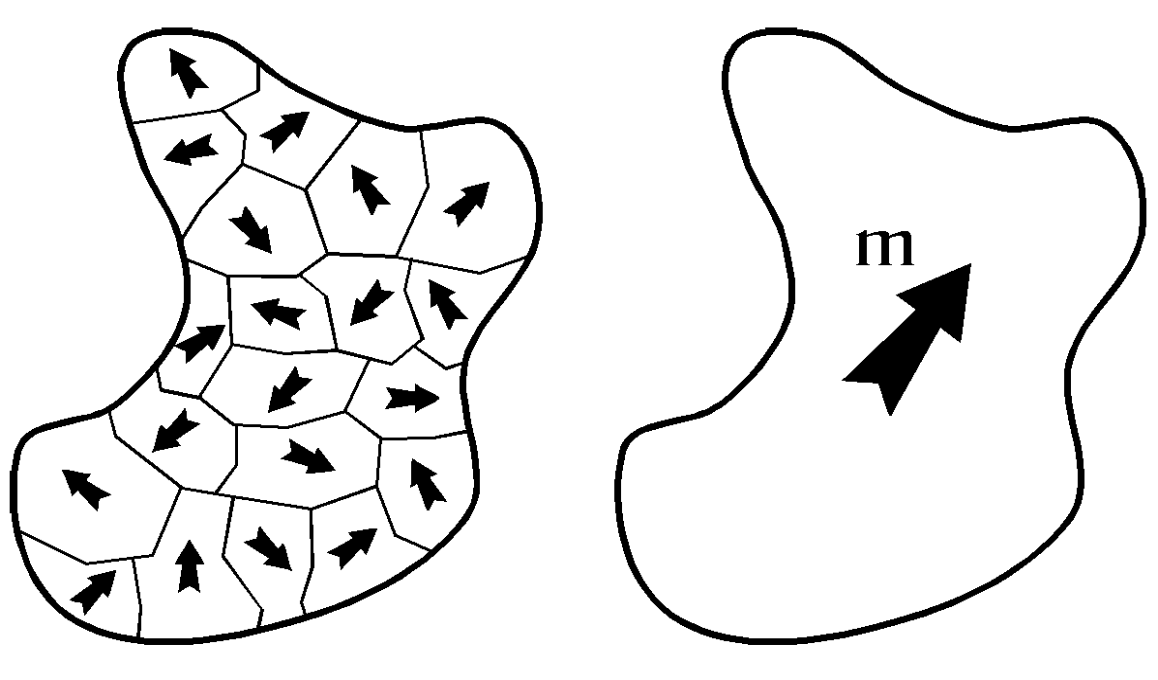
\includegraphics[width=0.35\textwidth]{Chapter_4/v4-domains}
    \caption{Доменная структура ферромагнетика при слабом (слева)
    и сильном (справа) внешнем поле}
    \figmark{domains}
\end{wrapfigure}

С другой стороны, магнитное диполь-дипольное взаимодействие между доменами препятствуют
выстраиванию всех магнитных моментов среды в одном направлении.
Действительно, энергия такого взаимодействия будет минимальной
при \important{анти}параллельном расположении магнитных моментов соседних элементов среды.
Поэтому при определённом поперечном размере домена оказывается
энергетически выгодно иметь соседний домен с противоположно ориентированным моментом
(см. рис.~\figref{domains}, слева).
Наложение внешнего поля заставляет домены ориентироваться
по нему, что приводит к резкому увеличению намагниченности образца, а при
достаточно большом поле достигается состояние \term{насыщения},
когда все домены ориентируются по полю (см. рис.~\figref{domains}, справа).

% Между доменами существуют переходные слои (в железе их толщина $\sim
% 10^{-5}$~см), в которых направление магнитного момента атомов плавно переходит
% от направления в одном домене к направлению в соседнем. Такие слои называют
% «стенками Блоха». Энергия этих слоёв пропорциональна их площади.
% \todo [author=Tiffani]{Неплохо было бы выделять термины вроде «стенками Блоха» и
% «скачки Баркгаузена» курсивом или жирным шрифтом при первом упоминании в
% тексте.}

\introsection{Ферромагнитный гистерезис}
\label{sec:histeresis}

Если состояние некоторой системы зависит не только от мгновенных значений
внешних параметров, но от истории их изменений, говорят, что
в системы имеет место \term{гистерезис}.

Именно такими свойствами обладает магнитный момент ферромагнитного образца
как функция напряжённости поля $M(H)$. В частности,
система может оказаться намагниченной, даже когда внешнее поле выключено ---
этим объясняется существование постоянных магнитов. Рассмотрим данное явление подробнее.

\paragraph{Кривая намагничивания}
Пусть ферромагнетик находится исходно в ненамагниченном состоянии
($M = 0$). Медленно увеличивая поле $H$ в образце, получим зависимость
$M(H)$, которую называют \important{начальной кривой намагничивания}. Эту кривую обычно
разделяют на пять условных участков (рис.~\figref{magnetization curve}).

Участок~1~--- область \emph{обратимого} намагничивания, где $M =\chi H$. В этой области
происходят процессы упругого смещения границ доменов: увеличивается размер тех
доменов, магнитный момент которых близок к направлению магнитного поля, и
уменьшаются размеры доменов с противоположным направлением магнитного момента.

\begin{wrapfigure}[]{r}{0.5\textwidth}
\centering\pic{0.5\textwidth}{Chapter_4/v4_3}
    \caption{Начальная кривая намагничивания ферромагнетика}
    \figmark{magnetization curve}
\end{wrapfigure}

Участок~2 характеризуется квадратичной зависимостью $M$ от $H$. В этой области
также идёт процесс обратимого смещения границ, но проявляется нелинейный характер
зависимости намагниченности от поля.

Область максимальной скорости роста намагниченности 3 соответствует 
\emph{необратимым} смещениям стенок между доменами (<<стенок Блоха>>):
им приходится преодолевать <<препятствия>> в виде примесей,
дислокаций и дефектов кристаллической решётки.
Когда стенка наталкивается на такое препятствие, она останавливается и держится,
пока поле не достигнет порогового значения, при котором она внезапно
срывается. Таким образом, движение доменной стенки приобретает скачкообразный
характер (<<скачки Баркгаузена>>).

% Фрагмент кривой намагничивания в этой области в увеличенном масштабе показан на
% рис.~\figref{magnetization curve}. Скачкообразное движение стенок приводит к
% быстрому изменению намагниченности образца, что вызывает появление вихревых
% токов, а следовательно, диссипацию энергии. Выделение тепла внутри образца и
% приводит к необратимому движению доменных стенок.

В достаточно сильных полях движение стенок прекращается и энергетически
выгодным становится поворот магнитных моментов тех оставшихся доменов, у которых
магнитный момент не совпадает с направлением поля (область 4).

И, наконец, при некотором значении поля (участок 5) все магнитные моменты
выстраиваются по полю~--- намагниченность образца достигает 
\emph{насыщения} ($M=M_s$).

% Повторы! // ППВ
%
% \begin{wrapfigure}[12]{r}{0.35\textwidth}
% 	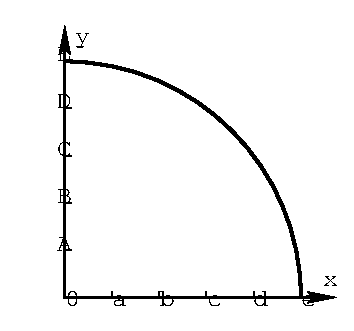
\includegraphics[width=0.2\textwidth]{v4_4}
% 	\caption{Зависимость намагниченности насыщения ферромагнетика от
% температуры}
% 	\figmark{magnetization-temperature}
% \end{wrapfigure}
%
% Магнитные и другие физические свойства ферромагнетиков существенным образом
% зависят от температуры. Например, намагниченность насыщения $M_s$ имеет
% наибольшее значение при $T = 0~(M_s (0))$ и монотонно уменьшается до нуля при
% температуре $\Theta$, которую называют ферромагнитной точкой Кюри
% (рис.~\figref{magnetization-temperature}).
%
% \todo [author=Tiffani]{Обозначения на рис. 4.4 не имеют ничего общего с
% действительностью.}
%
% Выше  этой температуры $\Theta$ тепловое движение разупорядочивает магнитную
% структуру доменов и ферромагнетик переходит в парамагнитное состояние. В
% отсутствие внешнего магнитного поля переход ферромагнетик~---парамагнетик
% является фазовым переходом II рода.
%
% Мы уже знаем, что для парамагнетиков зависимость магнитной восприимчивости от
% температуры имеет вид закона Кюри ($\chi \sim 1/T$). Аналогичная зависимость
% восприимчивости ферромагнетиков от температуры при температурах выше $\Theta$
% описывается законом Кюри-Вейсса:
% \begin{equation*}
% 	\chi = \frac{C}{T - \Theta_p},
% \end{equation*}
% где $C$ -- постоянная Кюри, $\Theta_p$ -- температура Кюри (как правило
% $\Theta_p > 0$).

На практике магнитные свойства ферромагнетиков обычно изучают путём измерения
зависимости индукции магнитного поля $B$ 
от напряжённости магнитного поля $H$ в веществе. 
Исследование образца обычно начинают 
с полностью размагниченного состояния 
($H = 0$, $B = 0$). Если монотонно увеличивать напряжённость~$H$, 
то изменение~$B$ происходит по рассмотренной выше
начальной кривой намагничивания с учётом соотношения \eqref{fieldB}:
$B(H)=\mu_0 (H+M(H))$ (кривая OA на рис.~\figref{hysteresis curve}).

Наклон кривой намагничивания характеризуется
\term{дифференциальной магнитной проницаемостью}
\begin{equation}
    \eqmark{mu-diff}
    \mu_{\text{диф}} \equiv \frac{1}{\mu_0} \frac{dB}{dH}.
\end{equation}
С ростом $H$ величина $\mu_{диф}$ сначала растёт 
(этом соответствуют участки~1 и~2 на рис.~\figref{magnetization curve}),
затем (с середины участка 3) начинает резко падать,
приближаясь к единице при насыщении.

\begin{figure}[h!]
    \centering
    \pic{60mm}{Chapter_4/v4_8}
    \caption{Начальная кривая намагничивания (OA) и предельная петля гистерезиса}
    \figmark{hysteresis curve}
\end{figure}

\paragraph{Явление гистерезиса}

Доведём систему до некоторой точки $A$, лежащей в области
насыщения (здесь $B_s$~--- \term{индукция насыщения}\footnote[1]{s~--- saturated
(англ.)~--- насыщенный}), и начнём уменьшать напряжённость~$H$.
Поскольку между доменами есть трение, обратный путь
пойдёт не по начальной кривой, а \emph{выше} неё.

При выключения внешних полей, то есть при достижении $H = 0$,
в образце сохраняется некоторое собственное намагничивание.
Соответствующее значение индукции $B_r$
называют \term{остаточной индукцей}\footnote[2]{r~--- remained (англ.)~--- оставшийся}.

Значение $B = 0$ достигается лишь при некотором отрицательном значении
$H = - H_c$. Величина $H_c$ называется
\term{коэрцитивным полем}\footnote[3]{c~--- coercive (англ.)~--- принудительный}.
Среди ферромагнетиков принято различать \important{магнитомягкие} 
($H_c \lesssim 1\;кА/м$) и \important{магнитожёсткие} ($H_c > 10$~кА/м) материалы. 
В точке~$C$ наступает насыщение для намагничивания в противоположную сторону.

Если теперь попробовать вернуться в точку $A$, вновь наращивая поле,
получим некоторый замкнутый цикл (предельную \term{петлю гистерезиса}). Если
в точке $A$ насыщение не достигается, то аналогичным образом  получится
цикл меньшей площади.

Отметим, что \important{площадь петли} гистерезиса ферромагнетика на плоскости
$H$--$B$ есть энергия, \emph{необратимо} выделяющейся в виде 
тепла в единице объёма вещества за один цикл:
\begin{equation}
    \eqmark{HdB}
    \Delta w = -\oint {HdB}
\end{equation}
(см. далее вывод формулы \eqref{magnetic-energy}).

% Можно короче. // ППВ
%
% Магнитное состояние вещества
% характеризуется теперь точками кривой $CA$, лежащими низке начальной кривой
% намагничивания. Строго говоря, кривая не пройдёт и через точку $A$, а окажется
% ниже неё. Вновь уменьшая магнитное поле, мы пройдём поэтому по кривой,
% расположенной ниже кривой $AC$, не попадём в точку $C$ и начнём движение к $A$
% по некоторому новому пути. Магнитные циклы, таким образом, обычно оказываются
% незамкнутыми. Многократно проходя один и тот же цикл, образец приближается к
% предельному замкнутому циклу (кривой гистерезиса), не зависящему от начального
% состояния. Описанная картина наиболее отчётливо проявляется в тех случаях, когда
% образец не доводится до насыщения. При заходе в область насыщения намагничивание
% зависит главным образом от $H$ и лишь в очень слабой степени от истории образца.
% Предельные циклы устанавливаются при этом сразу (т. е. при однократном
% прохождении цикла) или почти сразу. В соответствии с этим на
% рис.~\figref{magnetization curve} не сделано различия между частным циклом и
% предельным.


\introsection{Измерение напряжённости и индукции магнитного поля}
\label{sec:measure-HB}

\introsubsection{Размагничивающий фактор}

Когда говорят о кривой намагничивания $B(H)$,
речь идёт о \important{локальной} связи между
индукцией и напряжённостью магнитного поля в каждой точке среды.
При этом под $H$ имеется в виду не внешнее магнитное поле,
а именно поле \important{внутри} данного материала. Поскольку непосредственному
измерению легче всего поддаётся именно внешнее поле $\vec{H}_{0}$,
создаваемое сторонними токами без образца, необходимо установить связь
между $\vec{H}$ и $\vec{H}_0$ (заметим, что $\vec{B}_0=\vec{H}_0$).

Из условия непрерывности касательной компоненты вектора $\vec{H}$ следует,
что $\vec{H}$ совпадает $\vec{H}_{0}$ только если во всех точках образца
$\vec{H} \parallel \vec{H}_{0}$.
Такое возможно, например, в пределе \important{бесконечно длинного соленоида} либо
для \important{тонкого тора}.
В общем случае $\vec{H}_0 \ne \vec{H}$.

Рассмотрим магнетик, помещённый в однородное внешнее поле $\vec{H}_0$.
Разность между внешним полем и полем в образце принято называть
\term{размагничивающим полем}:
$\vec{H}_{разм} = \vec{H}_0 - \vec{H}$.
Если форма образца такова, что его намагниченность можно считать
практически постоянной $\vec{M}\approx\mathrm{const}$ (за исключением,
возможно, незначительных ``краевых эффектов''), можно ввести
коэффициент пропорциональности между $\vec{H}_{разм}$ и намагниченностью $\vec{M}$,
называемый \term{размагничивающим фактором}:
\begin{equation*}
N_{разм} = \frac{H_0-H}{M}.
\end{equation*}
Для однородного образца размагничивающий фактор зависит
только от его формы и ориентации в поле.
С учётом \eqref{fieldB} нетрудно убедиться, что его величина может меняться в пределах $0\le N_{разм} \le 1$.

Для образца с известным $N_{разм}$, изготовленного из материала
c проницаемостью $\chi$, помещённого во внешнее поле $H_0$, имеем
$H_0 - H = N M$, $M=\chi H$, откуда
\begin{equation*}
M = \frac{\chi H_0}{1+N_{разм}\chi}.
\end{equation*}

Аналитические выражения для $N_{разм}$ могут быть получены только для тел
простейшей формы. В частности
\begin{itemize}
    \item бесконечно длинный цилиндр: продольное поле~--- $N_{разм} = 0$,
          поперечное поле~--- $N_{разм} = 1/2$;
    \item шар $N_{разм} = 1/3$;
    \item бесконечно тонкая пластинка в поперечном поле $N_{разм} = 1$,
          в продольном --- $N_{разм} = 0$.
\end{itemize}

Заметим, что для диа- и парамагнетиков $|\chi|\ll 1$, поэтому отличием $H$ от
$H_0$ для них можно, как правило, пренебречь.

% Сложно и ненужно // ППВ
%
% На практике
% для снятия петли гистерезиса мы обычно помещаем во внешнее однородное магнитное
% поле ферромагнитный образец, имеющий конечные размеры. Однородная
% намагниченность по всему объёму образца будет иметь место только для образцов,
% имеющих форму эллипсоидов вращения, в частности, для шара, для очень тонкой
% пластинки и для тонкого и длинного цилиндра. Во всех этих случаях величина
% магнитного поля внутри образца будет меньше внешнего магнитного поля. Рассмотрим
% в качестве примера образец, имеющий форму цилиндра длиной $l$ и диаметром $d (d
% \ll l)$.
%
% Пусть ось симметрии цилиндра направлена вдоль внешнего магнитного поля величиной
% $H_0$. Цилиндр будет практически однородно намагничен с некоторой
% намагниченностью $M$. Найдём величину индукции магнитного поля на оси цилиндра в
% точке, равноудалённой от торцов. С одной стороны, используя связь между $B$, $M$
% и $H$, можно записать
% \begin{equation}
% 	\eqmark{cylinder-B(H)}
% 	B_{\text{вн}} = \mu_0 (H_{\text{вн}} + M),
% \end{equation}
% где $H_{\text{вн}}$~--- величина поля внутри образца. С другой стороны,
% намагниченный цилиндр можно рассматривать как цилиндрическую поверхность
% диаметра $d$ с однородным кольцевым поверхностным током плотностью:
% \begin{equation*}
% 	j = M.
% \end{equation*}
% Эти молекулярные токи создают собственное магнитное поле, которое по направлению
% совпадает с внешним полем $H_0$, а по величине равно\footnote[4]{См. [4]. Задача
% № 5.5.}:
%
% \todo [author=Tiffani]{Возможно, лучше вместо ``См. [4]. Задача № 5.5.''
% написать ``См. в приложении'', т.к. задача будет в приложении к этой главе}
% \begin{equation*}
% 	H_{\text{мол}} = \frac{Ml}{\sqrt{l^2 + d^2}}.
% \end{equation*}
%
% Индукцию магнитного поля найдём как суперпозицию внешнего поля и поля
% молекулярных токов:
% \begin{equation}
% 	\eqmark{B(H)-molecular current}
% 	B_{\text{вн}} = \mu_0\left( H_0 + \frac{Ml}{\sqrt{l^2 + d^2}} \right).
% \end{equation}
% Приравнивая \eqref{cylinder-B(H)} и \eqref{B(H)-molecular current}, получим
% \begin{equation*}
% 	H_0 + \frac{Ml}{\sqrt{l^2 + d^2}} = H_{\text{вн}} + M.
% \end{equation*}
%
% Разность между внешним и внутренним полями называют размагничивающим полем:
% \begin{equation*}
% 	H_{\text{разм}} = H_0 - H_{\text{вн}} = \left( 1 - \frac{1}{\sqrt{1 + \left(
% \frac{d}{l} \right)^2}} \right) M = N_p M.
% \end{equation*}
% И тогда связь поля внутри и поля внешнего
% \begin{equation*}
% 	H_{\text{вн}} = \frac{H_0}{1 + N_p M},
% \end{equation*}
% а  магнитная проницаемость образца
% \begin{equation*}
% 	\chi_{\text{обр}} = \frac{\chi}{1 + N_p \chi}.
% \end{equation*}
% \term{Коэффициент пропорциональности между размагничивающим полем и
% намагниченностью образца обозначают через $N_p$ и называют размагничивающим
% фактором или коэффициентом размагничивания. Его величина зависит только от
% геометрических размеров образца и может изменяться в пределах от 0 до 1.}

% Полученное выражение для $N_p$ цилиндра с параметрами $d/l \ll 1$ всё равно
% остаётся приближённым выражением, хотя и с достаточно хорошим приближением. А
% вот точные значения размагничивающего фактора могут быть рассчитаны только в
% отдельных частных случаях:

\introsubsection{Измерения в тороидальном образце}

\begin{wrapfigure}{o}{0.35\textwidth}
    \centering
    \pic{28mm}{Chapter_4/v4_5}
    \caption{Тороидальный образец с намагничивающей обмоткой}
    \figmark{toroid}
\end{wrapfigure}

В лабораторных условиях для исследования зависимости $B(H)$ ферромагнитных
материалов обычно используют образцы тороидальной формы. Если на тор намотать
равномерную намагничивающую обмотку (рис.~\figref{toroid}), то поле~$H$ внутри
тора на окружности радиуса~$R$ будет пропорционально току~$I$ в обмотке, а его
величину можно рассчитать по теореме о циркуляции вектора~$H$:
\begin{equation}
    \eqmark{H-toroid}
    H = \frac{IN_0}{2\pi R},
\end{equation}
где $N_0$~--- число витков намагничивающей обмотки. Напряжённость магнитного
поля в тороидальном образце зависит от $R$, поэтому
намагниченность образца можно считать однородной при $r \ll R$, где $r$ ---
радиус сечения тора.

\introsubsection{Поле в зазоре электромагнита}

\begin{wrapfigure}{o}{0.35\textwidth}
    \centering
    \pic{28mm}{Chapter_4/v4_6}
    \caption{Тороидальная катушка с разрезом}
    \figmark{toroidal coil-cut}
\end{wrapfigure}

Рассмотрим теперь тороидальную катушку, в которой сделан узкий разрез толщиной
$\delta$ ($\delta \ll r \ll R$) (рис.~\figref{toroidal coil-cut}).

Пусть $H_1$~--- напряжённость магнитного поля в
образце, а $H_2$~--- в зазоре. По теореме о циркуляции вектора $H$ имеем
\begin{equation}
	\eqmark{H-toroid-cut}
	\oint {Hdl} = H_1 (2\pi R - \delta) + H_2 \delta  = N_0 I.
\end{equation}

Воспользуемся нeпрерывностью нормальных составляющих вектора магнитной
индукции $B$ на границах разреза. В образце имеем $B_1 = \mu_0 \mu H_1$,
а в зазоре $B_2 = \mu_0 H_2$, поэтому приравнивая $B_1$ и $B_2$, найдём:
\begin{equation*}H_2 = \mu H_1.\end{equation*}
Подставляя это в \eqref{H-toroid-cut}, получим
\begin{equation}
	\eqmark{H1-toroid-inside}
	H_1 = \frac{N_0 I}{2\pi R + (\mu - 1)\delta},\quad H_2 = \mu H_1
\end{equation}
Отметим, прежде всего, что напряжённости поля в образце и в зазоре
(при $\mu = \mathrm{const}$) пропорциональны силе намагничивающего тока.
После того, как установлена величина коэффициента
пропорциональности, измерение напряжённости может быть заменено измерением тока.

При наличии даже небольшого зазора второе слагаемое в знаменателе
\eqref{H1-toroid-inside} может существенно превосходить первое из-за большой величины
$\mu\gg1$. Тогда полагая $\mu\gg \frac{2\pi R}{\delta}\gg 1$, из
\eqref{H-toroid-cut} найдём поле в зазоре:
\begin{equation}
	\eqmark{H2-toroid-big gap}
	H_2 \approx \frac{N_0 I}{\delta}.
\end{equation}
Интересно, что из \eqref{H2-toroid-big gap} следует, что поле в зазоре
электромагнита практически не зависит ни от размеров и формы магнитного ярма (части
магнитной цепи, заполненной веществом с большим $\mu$), ни от его материала.

% Воздушные зазоры электромагнитов можно использовать для исследования
% ферромагнитных образцов. А можно и не использовать.


\introsubsection{Измерение индукции в образце}

Один из простейших и в то же время надёжных методов измерения
индукции $B$ внутри некоторого образца основан
на законе электромагнитной индукции.
Электродвижущая сила, возникающая в контуре при изменении
пронизывающего контур магнитного потока $\Phi(B)$, равна
\begin{equation}
	\eqmark{EMF-magnetic flux}
	\mathcal{E} = - \frac{d\Phi (B)}{dt},
\end{equation}
Так как магнитный поток $\Phi (B)=BS$ равен произведению индукции $B$ на площадь
образца $S$, формула \eqref{EMF-magnetic flux} позволяет определить производную от
индукции $B$. Чтобы измерить саму величину $B=-\frac1{S}\int \mathcal{E} dt$,
необходимо иметь некоторое интегрирующее устройство.
В качестве такового может быть применён милливеберметр 
(работа \ref{lab:4-1}),
баллистический гальванометр (работа \ref{lab:4-4}), интегрирующая $RC$-цепочка
(работа \ref{lab:4-5}). 
В современной практике в основном применяется цифровое интегрирование.

\begin{lab:note}
Следует обратить внимание, что при измерениях в переменном поле
в образцах с большим $\mu$ и высокой электропроводностью
нельзя не учитывать конечную глубину
проникновения поля в образец из-за \emph{скин-эффекта}, равную
\begin{equation*}
\delta_{скин} \sim \sqrt{\frac{\rho}{\mu \mu_0 f}},
\end{equation*}
(cм. \textit{Сивухин Д.В.} Общий курс физики, Т.~3, \S 144.).
Здесь $\rho$~--- удельное сопротивление, $f$~--- частота колебаний поля.
Например, при $f=50\;Гц$ для чистого железа ($\rho \approx 10^{-7}\;Ом\cdot м$,
$\mu \sim 10^3$) имеем $\delta \sim 1\;мм$.
\end{lab:note}

\introsection{Энергия и силы в магнитном поле}
\label{sec:forces}

\introsubsection{Энергия поля}

Рассмотрим соленоид длиной $l$, площадью $S$ и числом витков $N$,
заполненный магнетиком с известным законом зависимости индукции от напряжённости
поля $B(H)$ (или $H(B)$). Подключим соленоид к источнику ЭДС~$\mathcal{E}$.
Пусть омическое сопротивление цепи равно $R$.
Плавно (квазистатически) увеличим ток в цепи до некоторого значения
$I$, так что напряжённость в соленоиде станет равна
$H = \frac{N}{l} I$. Закон Ома в цепи соленоида имеет вид
\begin{equation}
    \eqmark{OhmLaw-solenoid}
\mathcal{E} - IR = \frac{d\Phi}{dt},
\end{equation}
где правая часть отвечает ЭДС индукции, $\Phi = NBS$ --- магнитный поток в
цепи.

Магнитная энергия $W_М$, запасённая в соленоиде, равна работе
источника $A_{ист}=\int \mathcal{E}I\, dt$ за вычетом тепловыделения $Q=\int I^2 R\, dt$.
С~учётом \eqref{OhmLaw-solenoid}, получим
\begin{equation}
    \eqmark{magnetic-energy-full}
W_М = \int\limits_0^t I(\mathcal{E} - I R) dt =
\int\limits_0^t I\frac{d\Phi}{dt} dt = \int I\,d\Phi.
\end{equation}
В последнем равенстве мы перешли от интегрирования
по времени к интегрированию по значениям $\Phi$. Если связь между потоком и током
\important{линейна}: $\Phi = L I$, где $L=\mathrm{const}$ --- индуктивность, то
справедлива обычная формула для магнитной энергии
\begin{equation}
    \eqmark{magnetic-energy-full-simple}
    W_М = \frac{LI^2}{2} = \frac{\Phi I}{2} = \frac{\Phi^2}{2 L}.
\end{equation}


В случае произвольной геометрии магнетик
можно разбить на элементарные ячейки и определить
\term{объёмную плотность энергии} магнетика: разделив
\eqref{magnetic-energy-full} на объём $V=Sl$ и воспользовавшись соотношениями
$\Phi = NBS$ и $I=lH/N$, получим
\begin{equation}
    \eqmark{magnetic-energy}
 w_М = \int H\,dB.
\end{equation}
В частном случае простых диа- и парамагнетиков, для которых связь
$B=\mu \mu_0 H$ линейна, имеем упрощённую формулу
\begin{equation}
    \eqmark{magnetic-energy-simple}
    w_М = \frac{\mu\mu_0 H^2}{2} = \frac{HB}{2} = \frac{B^2}{2\mu\mu_0}
\end{equation}

Найдём изменение энергии \eqref{magnetic-energy} системы при переходе
по некоторому замкнутому контуру на плоскости $H$--$B$:
\begin{equation*}\Delta w_М = \oint H\,dB.\end{equation*}
Если все процессы в магнетике обратимы, то функция $H(B)$ будет
определена однозначно, и энергия будет сохраняться: $\Delta w_М =0$.
В ферромагнетиках имеет место гистерезис и функция $B(H)$ однозначной не является.
В таком случае в магнетике имеют место необратимые процессы, а величина
$\Delta w_М = \oint H\,dB <0$ (площадь петли) будет равна потерям энергии на тепловыделение
в образце за один период.

\introsubsection{Силы в магнитном поле}

Задача о силах, действующих на магнетики в магнитном поле, наиболее просто
решается энергетическим методом \important{виртуальных перемещений}.

Рассмотрим некоторую систему, находящуюся в равновесии,
для которой известна зависимость её магнитной энергии $W_М(x)$
от некоторой (обобщённой) координаты $x$. Пусть под действием
некоторой внешней силы $F$ (положительное направление по оси $x$)
система сместилась от равновесия на малую величину $\delta x$.
При этом сила совершила работу $\delta A = F\delta x$.
Эта работа может пойти на приращение магнитной энергии $\delta W_М$,
а также рассеяться в виде тепла $\delta Q$. Кроме того,
дополнительную работу может совершить источник $\delta A_{ист}$.
Таким образом, закон сохранения энергии имеет вид
\begin{equation*}
F\delta x = \delta W_М - \delta A_{ист} + \delta Q.
\end{equation*}

Предположим сперва, что магнитный поток в цепи поддерживается постоянным
($\Phi = \mathrm{const}$). Тогда из закона Ома \eqref{OhmLaw-solenoid}
в любой момент имеем $\mathcal{E} = IR$. Домножая на $I$, получим
$\mathcal{E} I = I^2R$,
то есть работа источника $\delta A_{ист}=\mathcal{E}Idt$
идёт целиком на тепловыделение $\delta Q=I^2Rdt$.
Значит, вся работа внешней силы пойдёт на приращение магнитной энергии:
$F \delta x = \delta W_М$. В таком случае внешняя сила равна производной
энергии системы по координате при  $\Phi=\mathrm{const}$ (или $B=\mathrm{const}$):
\begin{equation}
    \eqmark{force-Phi}
    F^{(внеш)}_x = \left(\frac{\partial W_М}{\partial x}\right)_{\Phi}.
\end{equation}

Пусть теперь поддерживается постоянным ток в цепи
($I = \mathrm{const}$). Здесь ситуация оказывается несколько сложнее.
Опять пользуясь законом Ома \eqref{OhmLaw-solenoid}, запишем:
\begin{equation*}
\delta A_{ист}-\delta Q=(\mathcal{E} I - I^2R) dt = I \delta \Phi
% =\delta Q + \delta W_М.
\end{equation*}
Видно, что вклад источника не учитывать нельзя (именно благодаря ему
ток поддерживается постоянным). Вычисления существенно
упрощаются, если мы имеем дело с материалами, для которых
реализуется \important{линейная} связь между $\Phi$ и $I$ (и между $H$ и $B$).
В таком случае из \eqref{magnetic-energy-full-simple} имеем
\begin{equation*}
\delta W_М|_{I=\const} = \delta\left(\frac{\Phi I}{2}\right) = \frac12 I \delta \Phi.
\end{equation*}
Видно, что вклад работы источника по модулю вдвое превосходит изменение
магнитной энергии и противоположен по знаку. Таким образом получаем
$F\delta x = \frac12 I\delta \Phi - I\delta \Phi = - \delta W_М$,
и внешняя сила равна производной
энергии системы по координате при  $I=\mathrm{const}$ (или $H=\mathrm{const}$),
\important{взятой с обратным знаком}:
\begin{equation}
    \eqmark{force-I}
    F^{(внеш)}_x = -\left(\frac{\partial W_М}{\partial x}\right)_{I}.
\end{equation}
Заметим, что полученная выше формула \eqref{force-Phi} более общая и
справедлива в том числе для ферромагнетиков с нелинейным законом
$H(B)$.
